%%% 左右余白が3cmもある. p1の上部の空白が数行分多い
\documentclass{interim} % 中間用 clsファイル
\usepackage[dvipdfmx]{graphicx}
\usepackage{amsmath}
\usepackage{comment}
\usepackage{amsfonts}
\chukantitle % タイトル

% タイトル
\date{2018年 7月 12日}
\thisevent{平成30年度 \  情報・ネットワーク工学専攻 \  コンピューターサイエンスプログラム \  修士論文発表会}
\title{動画像圧縮技術を用いた時系列分類手法の改良}
\mymajor{情報・ネットワーク工学専攻}
\mynum{1731154}
\mylab{古賀研究室}
\myname{村井 建応}

\renewcommand{\baselinestretch}{0.928}

\begin{document}
\maketitle

\section{はじめに}
近年,IoTの隆盛に伴い,時系列データを扱う事業が増加している.
時系列データの分類を手動で行うには人手や時間などコストがかかる.
そのため,時系列データの自動分類は重要な研究テーマである.
圧縮ベースの分類手法は,少ないパラメータで様々な分類問題に利用できるなどの点から注目されている.
圧縮ベース時系列分類手法の1つに,Recurrence Plots Compression Distance (RPCD)という手法がある\cite{RP}.
本研究では,RPCD手法に対して,分類精度の向上を目的とし,次の2点を達成した.
\begin{itemize}
	\item MPEG-1のq値というパラメータがRPCD手法の分類精度に影響を与えることを発見した.
	\item 最適なq値を設定することにより従来手法に対し分類精度を平均3\%強向上した.
\end{itemize}
\section{RPCD}
本章では,Recurrence Plots Compression Distance (RPCD)手法について述べる.
RPCD手法は,汎用の圧縮アルゴリズムに手を加えることなく実装が可能であるため,その実装のしやすさという点で注目されている.
\par
RPCD手法の類似度計算の流れを図\ref{fig:RPCD}に示す.
まず,2つの時系列データからそれぞれRecurrence Plots (RP)と呼ばれる画像を生成する.
次に,得られた画像を組み合わせ,2枚のフレームからなる動画像を作成する.
得られた動画像をMPEG-1で圧縮し得られたファイルサイズから類似度を計算する.


\begin{figure}[t]
	\centering
	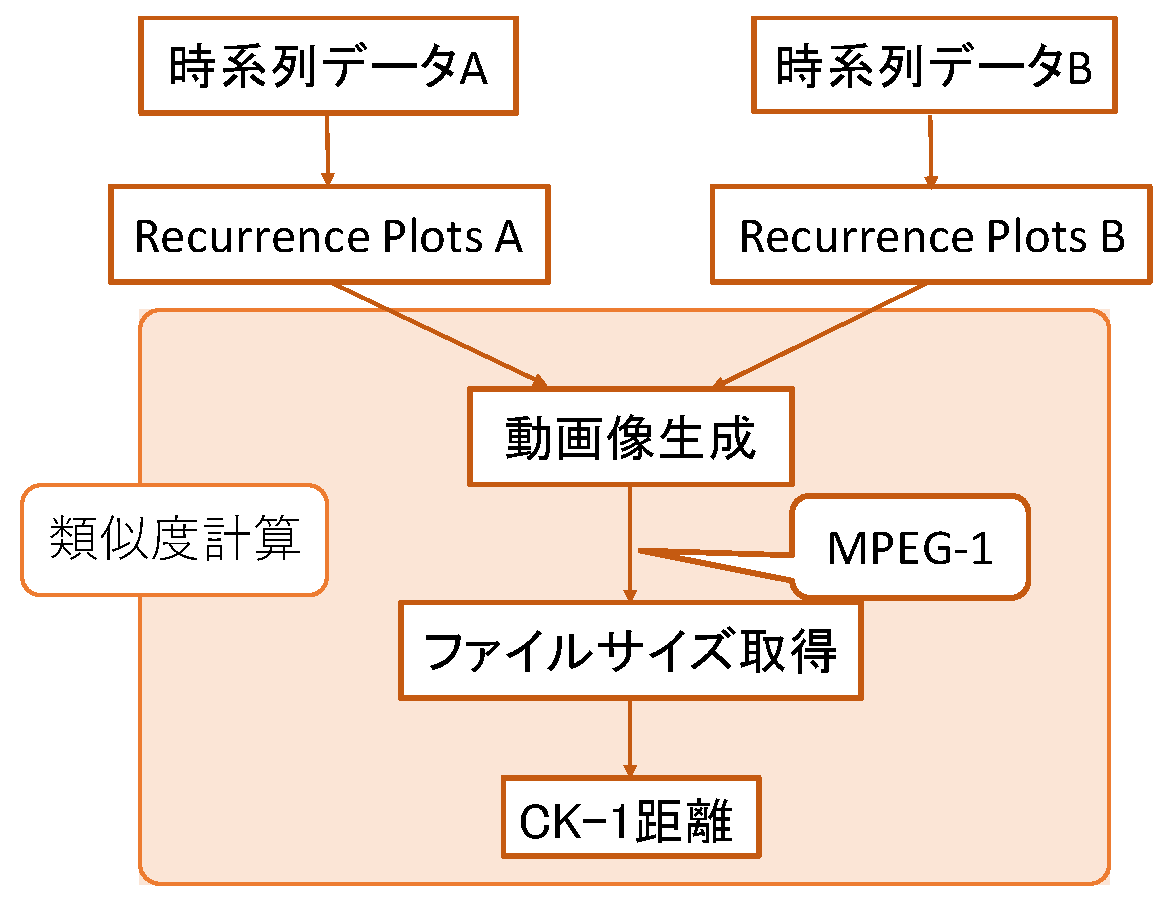
\includegraphics[width=7cm]{RPCD.eps}
	\caption{RPCD手法の流れ}
	\label{fig:RPCD}
\end{figure}
\subsection{Recurrence Plots}
Recurrence Plots (RP)は,時系列データの自己相関を表す図である.
RPは式(\ref{RP1})で表される.
\begin{eqnarray}
\label{RP1}
RP(i,j)=||\vec{x}(i)-\vec{x}(j)||, \vec{x}(\cdot)\in\mathbb{R}
\end{eqnarray}
ここで,$\vec{x}(i)$は時系列データ$x$の$i$番目のサブシーケンスを表す.
得られたRPを正規化し,$RP(i,j)$の値を画素位置$(i,j)$の画素値とみなすことでグレースケール画像として表現できる.

\subsection{MPEG-1}
MPEG-1は動画像圧縮規格の1つであり,1993年にISO/IEC 11172として標準化された.
MPEG-1では動き補償フレーム間予測を採用している.
動き補償フレーム間予測とは,圧縮対象のフレームの画素情報を直前のフレームの画素情報から予測して圧縮する方法である.
2枚のフレームが似ている場合,フレーム間の差分が小さくなるため,圧縮動画像のファイルサイズは小さくなる.
\subsection{CK-1距離}
CK-1距離はCampanaらによって定義された2つの画像間の距離を動画像圧縮技術を用いて測る方法である\cite{ck1}.
2つの画像$x$と$y$が与えられたとき,CK-1距離$D(x,y)$は式(\ref{CK-1})で定義される.
\begin{eqnarray}
\label{CK-1}
D(x,y)=\frac{C(x|y)+C(y|x)}{C(x|x)+C(y|y)}-1
\end{eqnarray}
ここで,$C(x|y)$は1枚目に画像$y$,2枚目に画像$x$の2フレームで構成される圧縮動画像のファイルサイズである.
画像$x$と画像$y$が同じ画像であった場合,$C(x|y),C(y|x),C(y|y)$は$C(x|x)$に等しくなりCK-1距離$D(x,y)=0$となる.


\section{q値のRPCD手法への影響}
本研究では,MPEG-1のq値というパラメータがRPCD手法を用いた時の分類精度に影響を与えることを発見した.
q値とは圧縮動画像の品質を決めるパラメータであり,量子化などに影響を与える.
q値が設定されていない場合,デフォルトで設定されている目標ビットレートに沿うよう,圧縮ソフト側でフレームごとに適応的に決定される.
この時,決定された品質によってファイルサイズが左右される.
RPCD手法は「2枚のフレームが似ているほどファイルサイズが小さくなる」MPEG-1圧縮の特性を活用した手法であるため,フレームごとに品質が異なると正しい分類が困難になる.
このことから,分類にはq値の固定が必要であると考えられる.
いくつかのq値で固定してRPCD手法を試したところ,q値によって分類精度が変わることが確認できた.
結果の一部を表\ref{table:q}に示す.
\begin{table}[b]
	\centering
	\caption{q値による分類精度の変化}
	\label{table:q}
	\small
	\begin{tabular}{lccc}
		\hline
		dataset&q=1&q=10&q=30\\
		\hline
		\hline
		50wrods&76.67&\bf{80.67}&78.89\\
		Cricket X&8.97&57.18&\bf{77.18}\\
		ECGFiveDays&\bf{91.30}&73.91&73.91\\
		\hline
	\end{tabular}
\end{table}
表\ref{table:q}より,データセットごとに最適なq値が異なることがわかる.

\section{qRPCD}
本研究では,教師データから最適q値をあらかじめ予測するqRPCD手法を提案する.
qPRCDでは,leave-one-out cross-validationにより教師データをRPCD手法で分類した精度から最適q値を予測する.
分類には1-NNを用いる.
最適q値の予測方法を示す.

\begin{itemize} 
	\item[1] 代表q値を1から100までの中から等間隔に選び,最も分類精度の高い代表q値を1つ選ぶ
	\item[2] 1で選択した代表q値の前後10個のq値において,最も分類精度の高いq値を最適q値とする
%	\item[3] 1,2で代表q値,最適q値に複数候補が見つかった場合,より小さいq値を代表q値,最適q値とする
\end{itemize}
代表q値の間隔は10と定めた.なお,選択する代表q値,最適q値に複数候補が見つかった場合,より小さいq値を選択する.
予測した最適q値を用いて,RPCD手法により類似度を計算する.

\section{実験および結果}
\subsection{実験方法}
UCR Time Series archiveから27個のデータセットを使用して,qRPCD手法と2つの従来手法 (RPCD,CRPCD)との分類精度を比較する.
CRPCD手法とは,2つの時系列データを組み合わせてRPを作成するCross Recurrence Plotsを用いて分類を行う手法である\cite{CRP}.
圧縮ソフトはFFmpegを用いてMPEG-1圧縮を行う.
分類には1-NNを用いる.
\subsection{結果}
qRPCD手法と2つの従来手法との分類精度の比較を行った.
結果を表\ref{ta:hikaku}に示す.
表\ref{ta:hikaku}より,qRPCD手法は27個のデータセット中,18個で最も良い分類精度であった.
また,平均分類精度は,RPCD手法に対し3\%強,CRPCD手法に対し4\%強の向上が見られた.
\begin{table}[t]
	\small
	\caption{分類精度}
	\label{ta:hikaku}
	\begin{tabular}{lccc}
		\hline
		dataset&RPCD&CRPCD&qRPCD\\
		\hline
		\hline
		50words&77.36&78.46&\bf{78.68}\\
		Adiac&61.64&61.38&\bf{71.10}\\
		Beef&\bf{63.33}&46.67&\bf{63.33}\\
		CinC ECG torso&97.90&93.19&\bf{97.97}\\
		Coffee&\bf{100}&85.71&\bf{100}\\
		Cricket X&70.77&\bf{75.64}&72.56\\
		Cricket Y&73.85&\bf{82.56}&73.85\\
		Cricket Z&70.77&\bf{77.69}&74.62\\
		DiatomSizeReduction&\bf{96.41}&96.08&94.12\\
		ECG200&86.00&\bf{88.00}&85.00\\
		ECGFiveDays&86.41&80.48&\bf{94.08}\\
		FISH&87.43&76.00&\bf{93.71}\\
		FaceFour&94.32&\bf{95.45}&94.32\\
		Gun Point&\bf{100}&98.67&\bf{100}\\
		Haptics&38.64&\bf{41.23}&39.94\\
		InlinseSkate&32.00&35.45&\bf{43.45}\\
		ItalyPoserDemand&84.26&83.77&\bf{94.27}\\
		Lighting2&75.41&\bf{81.97}&73.77\\
		Lighting7&64.38&\bfseries{69.86}&60.27\\
		MedicalImages&71.05&71.97&\bfseries{72.11}\\
		OSULeaf&64.46&65.29&\bfseries{85.12}\\
		OliveOil&83.33&73.33&\bfseries{86.67}\\
		SonyAIBORobot&79.70&79.70&\bfseries{87.35}\\
		SonyAIBORobotII&84.26&84.47&\bfseries{86.49}\\
		SwedishLeaf&90.24&88.80&\bfseries{91.20}\\
		Symbols&90.45&90.05&\bfseries{97.19}\\
		WordsSynonyms&72.41&73.35&\bfseries{77.59}\\
		\hline
		Best&4/27&8/27&\bf{18}/27\\
		Average&77.66&76.86&\bfseries{81.07}\\
		\hline
	\end{tabular}
\end{table}
精度が向上した要因として,適切なq値を設定することで量子化の際,ノイズとなる部分がうまく除去できたのではないかと考えられる.
また,9つのデータセットで分類精度の向上が見られなかった原因として,教師データの数が少ないデータセットにおいて,最適q値を十分に予測ができなかったことが考えられる.
\section{まとめと今後の課題}
本研究では,圧縮ベースの時系列分類の精度向上を目的として,q値がRPCD手法において分類精度に影響することを発見し,最適q値を予測するqRPCD手法を提案した.
qRPCD手法は,従来手法に対し平均して3\%強の分類精度向上を達成した.今後の課題として,q値によって分類精度が変化する原因の調査および,最適q値の予測方法の改善がある.
% 参考文献
\begin{thebibliography}{99}
	\scriptsize  % 参考文献以降の文字の大きさ
%\small
%	
	\bibitem{RP}
	G. D. B. Silva and V. de Souza, ``Time Series Classification using compression distance of recurrence plots,'' in Proc. IEEE 13th Int. Conf. Data mining, pp. 687-696, 2013.
	\bibitem{ck1}
		B. J. L. Campana and E. J. Keogh, ``A Compression Baseed Distance Measure for Texture,'' in Proc.  the 10th SIAM International Conference on Data Mining, pp. 850-861, 2010.
	\bibitem{CRP}
	T. Michael, S. Spiegel,and S. Albayrak, ``Time Series Classification using Compressed Recurrence Plots, '' in Proc. ECML-PKDD, pp. 178-187, 2015.
\end{thebibliography}
\end{document}